\documentclass[10pt,conference]{IEEEtran}
\IEEEoverridecommandlockouts
% The preceding line is only needed to identify funding in the first footnote. If that is unneeded, please comment it out.
\usepackage{cite}
\usepackage{amsmath,amssymb,amsfonts}
\usepackage{algorithmic}
\usepackage{graphicx}
\usepackage{textcomp}
\usepackage{xcolor}
\def\BibTeX{{\rm B\kern-.05em{\sc i\kern-.025em b}\kern-.08em
    T\kern-.1667em\lower.7ex\hbox{E}\kern-.125emX}}
\begin{document}

\title{Paper Title*\\
%{\footnotesize \textsuperscript{*}Note: Sub-titles are not captured in Xplore and
%should not be used}
%\thanks{Identify applicable funding agency here. If none, delete this.}
}
\author{\IEEEauthorblockN{1\textsuperscript{st} Given Name Surname}
\IEEEauthorblockA{\textit{dept. name of organization (of Aff.)} \\
\textit{name of organization (of Aff.)}\\
City, Country \\
email address}
\and
\IEEEauthorblockN{2\textsuperscript{nd} Given Name Surname}
\IEEEauthorblockA{\textit{dept. name of organization (of Aff.)} \\
\textit{name of organization (of Aff.)}\\
City, Country \\
email address}
\and
\IEEEauthorblockN{3\textsuperscript{rd} Given Name Surname}
\IEEEauthorblockA{\textit{dept. name of organization (of Aff.)} \\
\textit{name of organization (of Aff.)}\\
City, Country \\
email address}
}

\maketitle

\begin{abstract}
JavaScript is the most dominant language used to develop front-ends and back-end in multiple web applications. This is because of multiple features it brings with it along the lines of event-driven and asynchronous programming; which are one of the most crucial aspects when developing a smooth and fast web interface. One of the features that helps maintain flow of instructions in asynchronous language is callbacks or higher order functions. However, a poor understanding of callbacks can result in many complexities such as nested callbacks (also referred to as callback hell). Another problem that nested callbacks can cause is lose of benefit of asynchrony since execution of program becomes linear when independent functions are nested into callbacks of other function calls. We present a tool developed in JavaScript that checks for independent instructions inside callbacks and refactors them outside of callbacks.
\end{abstract}

\begin{IEEEkeywords}
JavaScript, Callbacks, Refactoring, Asynchronous programming
\end{IEEEkeywords}

\section{Introduction}
Callbacks if implemented rightly can result in a very smooth and robust functioning of program, however, callbacks in JavaScript are inherently difficult to understand. They get even more complicated when there are callbacks nested within other callbacks. In addition to increasing complexity in understanding code, they can also result in loss of benefits that JavaScript brings on table with its asynchronous way of executing instructions. Consider the code excerpt in figure 1, we see in line number 14 a call to readfile for file1.txt with a callback, in its callback there is another call to same function with file2.txt. Execution of this code will result in a completely serial reading of files, where as we could have achieved better results if second call was outside the callback of first call.
\begin{figure}[htbp]
	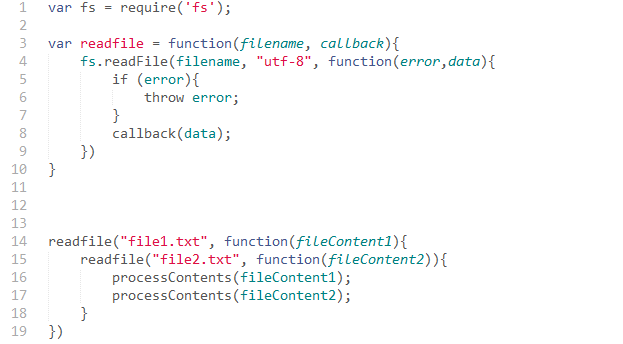
\includegraphics[scale=0.5]{introImg1.png}
	\caption{Example of a nested callback with independent instructions in callbacks}
	\label{fig}
\end{figure}

On average, every tenth function in JavaScript user applications takes a callback as an argument, over 43\% of these callback functions are anonymous and majority of these callbacks are nested \cite{b3}. This naturally means, there will be many such situations where callbacks will be affecting asynchrony and their refactoring will not result in any change in execution of program. This gives us opportunity to develop a method that automates refactoring in JavaScript function callbacks in such a way that independent instructions are taken out of callbacks and placed in a scope where their earlier execution does not affect functionality of program but enhances the overall performance.


Rest of the articles is divided into following order:
\begin{itemize}
	\item Methodology
	\item Implementation
	\item Testing
	\item Limitations and Challenges
	\item Related Work
	\item Conclusion

\end{itemize}

\section{Methodology}
Our proposed solution refactors all the independent instructions from callbacks, these can be reduced and limited to only async I/O or other blocking instruction but for simplicity we will currently refactor all independent instructions. Our solution mainly consists of 3 major parts:
\begin{itemize}
	\item AST extraction
	\item Execution context extraction
	\item Decision based refactoring
\end{itemize}
\subsection{AST extraction}
Abstract Syntax Tree is the context form of a parse tree that contains information about order of different instructions, operators and variables. An AST assigns a separate node to every operator or operand it encounters in code; thus, making a full fledge tree for the whole syntax of program. There are multiple different tools available that produce detailed AST for any given code. We can extract information like names of variables, scope of variables, structure of functions and metadata like line number in actual code etc. 

\subsection{Execution Context extraction}
Next, we use AST to develop execution context of our program. Execution context is the environment, different functions execute in. Typically, execution context contains information such as names of variables, scopes of variables, variables declared within a function and global variables. To extract execution context, we maintain dictionaries for different variables: for variables in scope of each function we maintain a separate dictionary, for variables declared in a function we have a separate dictionary and for arguments of function we have a different dictionary. We traverse the whole AST recursively from root to leaves and at each node we check if it’s a variable we append it to appropriate function’s list. At the end of this function we have complete execution context of the program. Pseudo code for Execution Context Extraction is shown in figure 2.

\begin{figure}[htbp]
	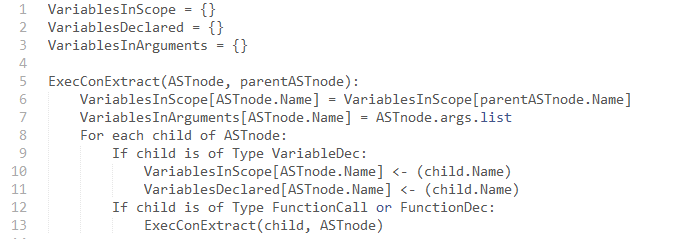
\includegraphics[scale=0.5]{code-execcon-extract.png}
	\caption{Pseudo code for Execution Context Extraction}
	\label{fig}
\end{figure}

\subsection{Decision based refactoring}
After we have execution context and we know scopes of different variables, we can now make decisions about what instructions are refactorable. We can refactor only a few types of instruction, the fact that what instructions are fit for refactoring depends upon what variables they depend upon. In this perspective we can have following 4 cases:
\begin{itemize}
	\item {\textbf{Instruction depends upon no variable:}
		There can be instructions that do not depend upon any of the variables for example declaration of a new variable, or line number 15 from figure 1 is fit to be refactored. In this case, instruction is safe to be refactored.}
	\item{\textbf{Instruction depends upon function argument:}Since callbacks may include instructions that are dependent upon arguments of main function, we should not refactor these instructions out of function.}
	\item{\textbf{Instructions depend upon variables declared in scope of parent function:}
		In this case, such an instruction will be safe to be refactored.}
	\item{\textbf{Instruction depends on a variable declared within the scope of function:}
		This case can have two scenarios, either the variable in terms of which the instruction is expressed is itself refactorable or it is not. In first case, when variable itself is refactorable, we can first let variable declaration instruction get refactored first and then refactor the instruction that contains the said variable.
		In other case when variable cannot be refactored, we do not refactor any instruction that contains it.}
\end{itemize}

\begin{figure}[htbp]
	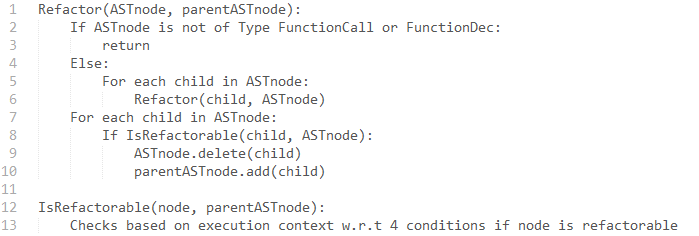
\includegraphics[scale=0.5]{code-decision-refactor.png}
	\caption{Pseudo code for Decision Based Refactoring}
	\label{fig}
\end{figure}

Now that we have mentioned decisions that will be governing decision of refactoring, we can move to actual methodology of refactoring. Refactoring function works recursively in bottom up manner, refactoring the deepest of callbacks first and then propagating refactoring towards the containing function. Figure 3 shows pseudo code for refactoring. For each node we recursively call refactor for every child and once all children nodes have been refactored we check for every child node with respect to fore-mentioned conditions if child node is refactorable. If it is refactorable, we delete that node from current tree node and add it to parent tree node.
\section{Implementation}
We have implemented above mentioned program in JavaScript ECMAScript 5 due to some constraints. We use UglifyJS to extract AST since it gives a very detailed tree with metadata such as line number and character number included within the tree. Additionally, it allows easy refactoring and is convertible to code even after we have made changes to tree. Moreover, UglifyJS also provide features such as tree compression and mangling variable names which can be helpful. Since UglifyJS is only compatible with JavaScript ECMAscript 5, we have also implemented our code in same version.

\section{Testing}
\section{Limitations and Challenges}
\section{Related Works}
Not a lot of work have been done regarding this specific problem. Following few pieces of work have some indirect relations with our work. 
\begin{itemize}
	\item {\textbf{Classification of Callbacks:}
		This paper does in depth analysis of 138 JavaScript pages with over 5 million 
		lines of codes. Study shows that around every 10th function takes a callback as an argument and 43\% of these callbacks are anonymous functions. Among these functions almost half are asynchronous calls. This shows importance of a tool that polices callbacks to ensure callbacks do not become too complicated \cite{b3}. 
	}
	\item{\textbf{Synchronous to Asynchronous:}
		Realizing the importance and usefulness of asynchronous programming, this work introduces way to convert to synchronous code of JavaScript to asynchronous to improve responsiveness of mobile apps \cite{b1}. 
	}
	\item{\textbf{Detecting JS code smells:}
		This paper does analysis of a sample of JavaScript programs and finds most common coding flaws. It presents a way of detecting these code smells. A notable code smell it talks about is nested callbacks, which can become hard to read and consequently debug. However, it only detects these code smells and does not provide any solution. Our work extends on this explicit problem and we try to cover a subset of problems caused by callbacks and try to solve \cite{b2}. 
	}
\end{itemize}
\section{Conclusion}
Callbacks can ensure very smooth and prompt execution of program if they are implemented rightly. However, since callbacks tend to get complex as they get nested they might even affect asynchrony of program execution. Our approach tends to find such abnormalities in JavaScript programs and improves performance by refactoring such instructions to position where they are executed earlier without affecting functionality of program. We achieve this goal by extracting AST of code using a JavaScript library UglifyJS, next we extract execution context from the AST and finally based on this AST and few rules we choose which instructions can be refactored. These instructions are removed from current function’s body and are placed in callee function’s body. Our approach currently only works on JavaScript ECMAscript 5 due to compatibility issues of UglifyJS, but it can be extended to newer versions if replacement for UglifyJS is found. 

\begin{thebibliography}{00}
\bibitem{b1} D. Dig ``Refactoring for asynchronous execution on mobile'' in IEEE Software, 2015.
\bibitem{b2} A.M. Fard and A. Mesbah "JSNOSE: detecting javaScript code smells" in IEEE 13th International Working Conference on Source Code Analysis and Manipulation (SCAM), 2013.
\bibitem{b3} G. Keheliya, A. Mesbah and B. Ivan "Don't call us, we'll call you: characterizing callbacks in javascript" in IEEE Empirical Software Engineering and Measurement (ESEM), 2015.
\end{thebibliography}


\end{document}
